\chapter{Summary and Conclusions}
\label{cp.conc}
In this thesis, I have XX.
I first provided a thorough overview of computational Bayesian analysis for gravitational-wave inference, introducing the software libraries underlying the bulk of the analysis in this thesis.
I then demonstrated GW151226...
These results tell us about astrophysics

In the last chapter of this thesis, I have illustrated a proof-of-concept design for the kind of science that may be facilitated by gravitational waves in the future, when conclusive measurements of mass and spin, and eccentricity will identify the AGN mergers in the population...

In the remainder of this thesis, I conclude with some thoughts about how this work should be improved and extended in the coming years.

\section{Infereing parameters of }

TESS, BCR, Pbilby, Deep Followup tell us about systems

\section{Population}
TESS AGN will tell us about populations


More detections will be possible, which also means more physics! 
\begin{figure}
\begin{center}
  \centerline{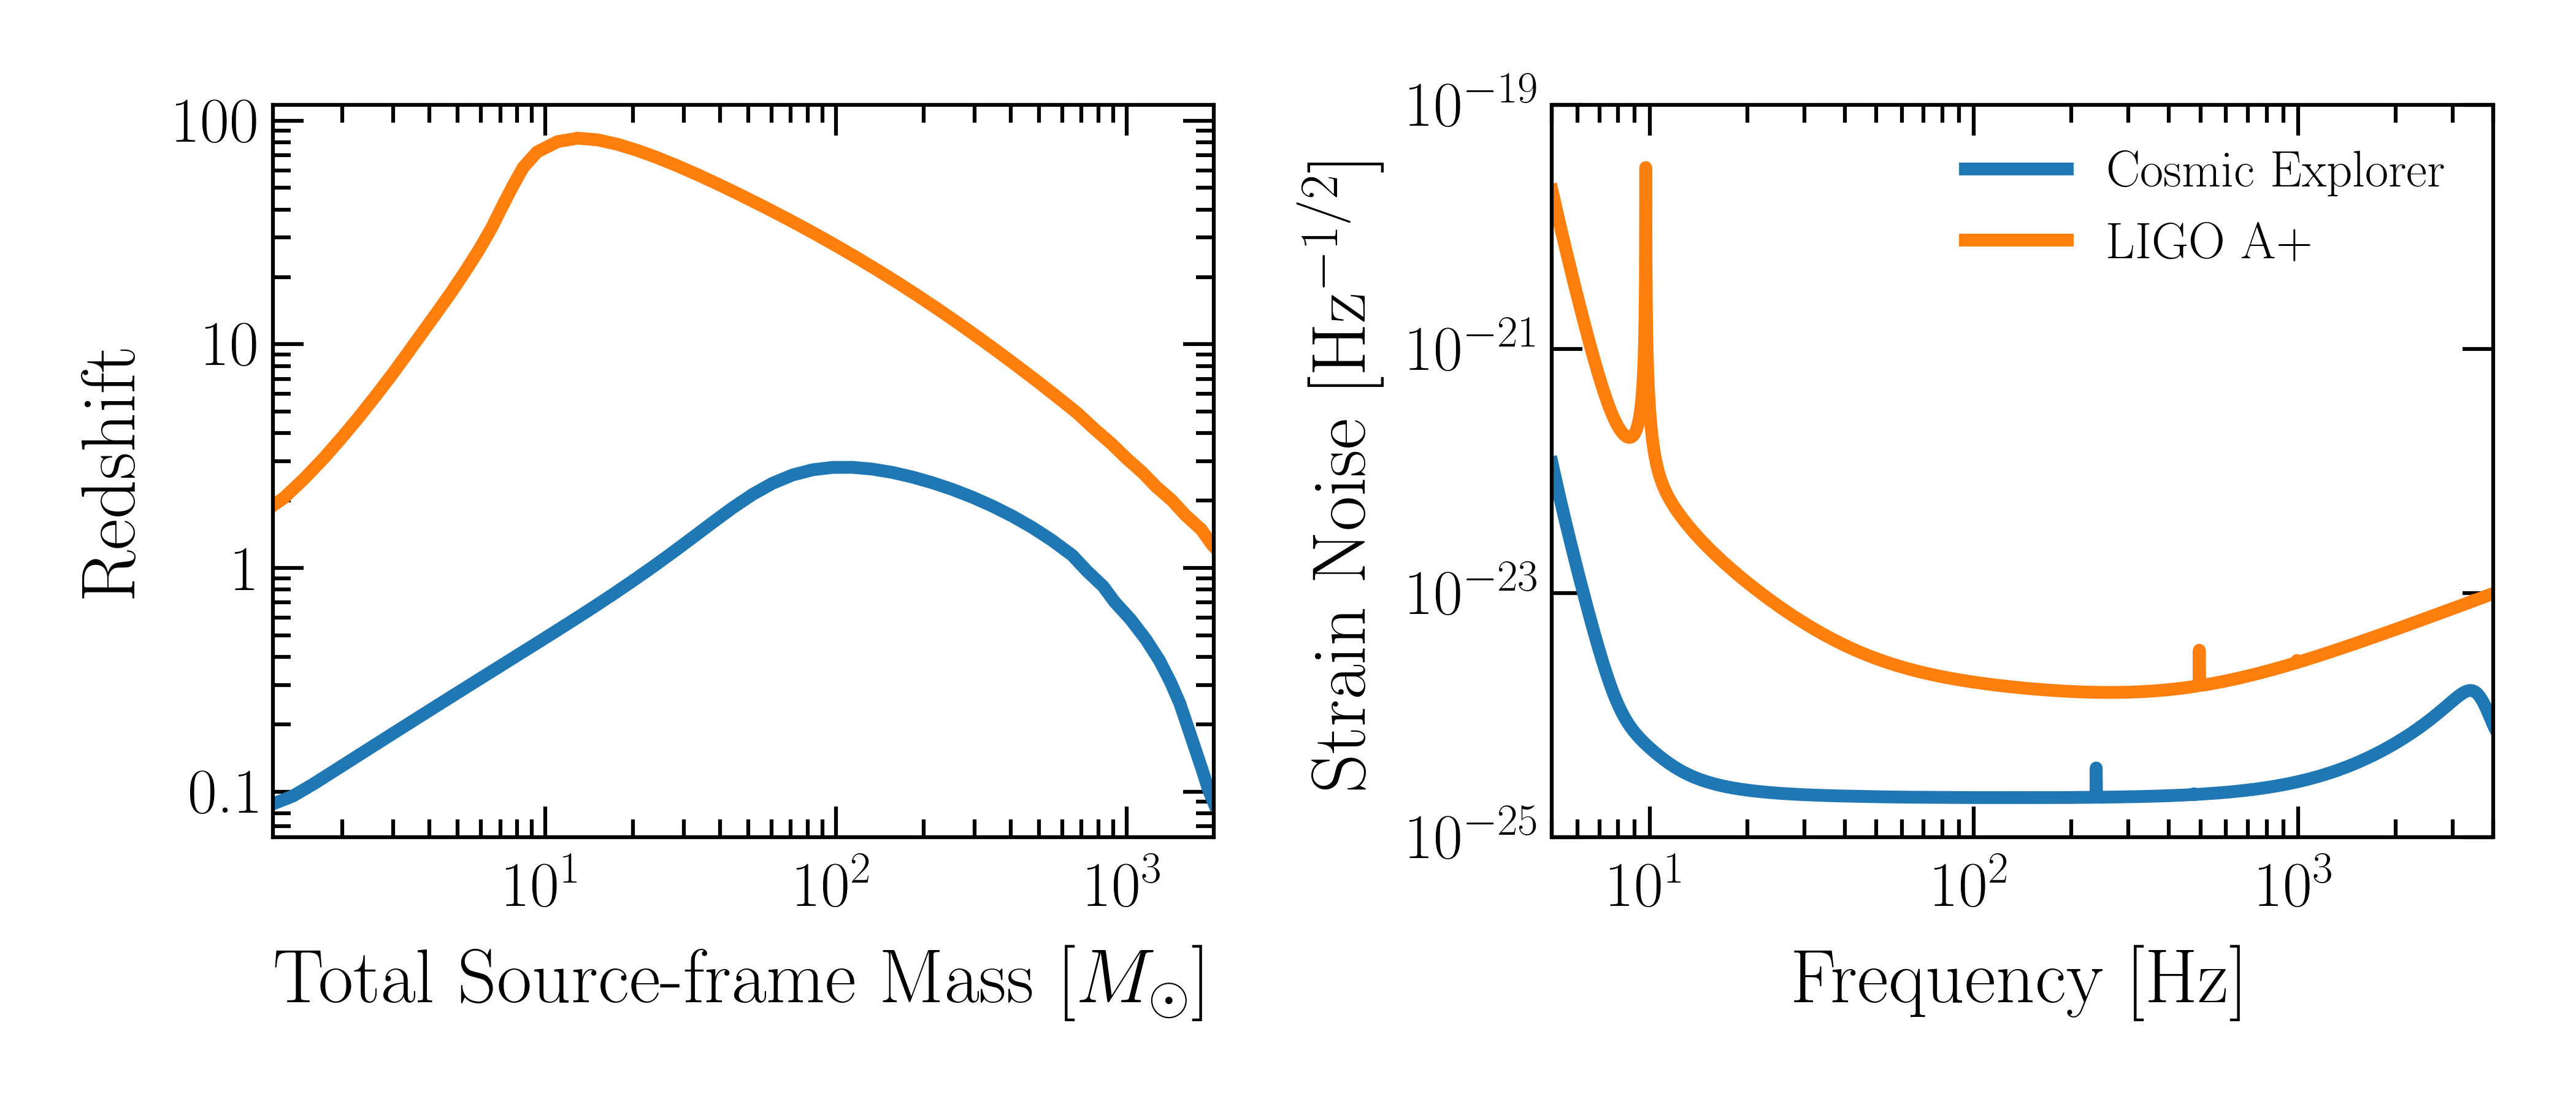
\includegraphics[width=1.\linewidth]{src/figures/ligo_vs_ce.png}}
  \caption{\textbf{LIGO A+ and CE Comparisons:}  \github{https://github.com/avivajpeyi/cbc_gw_catalog_plotter}}
  \label{fig:ligo_vs_ce}
\end{center}
\end{figure}



With an inordinate amount of data being produced using modern instruments, astronomy has become more data driven than ever before.


Modern astronomy finds its basis in the streams of data delivered by ground and space-based telescopes across all wavelengths with frontiers emerging in the field of neutrino physics, high-energy astrophysics, and gravitational waves.
With the enormous amount of data funnelling through the observational centres or high-end simulations, knowledge processing and accumulation in astronomy is growing exponentially.


An accelerating amount of data is now being received to help us understand the physical universe. With the advent of the internet age and the establishment of public data archives, we have also democratised data access and its processing. This coming of age in astronomy not only revolutionized it but also led to a paradigm shift in the nature of astronomical research and its method over the turn of the last century.



Evolving from location and laboratory-intensive research to global collaborative data-driven projects, the world has come quite far.  We are in the transition into the ever-evolving new. This also gives us an opportunity to archives, assess, and communicate the becoming of data-driven astronomy from the 1980s until now. It is the historicization of such intense research material over these decades that makes us understand the intellectual movement in the field but also helps us assess emerging fields like astroinformatics.  T
he gradual shift from analogue to digital observational methods led to the shift in data-collection regimes.
Astronomers have moved from photographic, and electronic, to born-digital data, which moved the discovery away from the telescope itself to hard drives and data archives. T
his not only becomes a study in the history of technology but also an intellectual history of knowledge networks and global collaborations.


In researching the cosmos, astrophysicists try to comprehend the vast scale of the universe, both spatial and temporally.


The next frontier for inquiry is characterizing the atmospheres of exoplanets. It's the next step toward finding life. Some scientists, especially Seager, are keen to peer into these atmospheres and look for the signs of living, breathing, metabolizing organisms.

Exoplanets have a similar driver larger than pure scientific curiosity. The ultimate goal
for many researchers is the search for habitable exoplanets. The exoplanet atmosphere
is the only way to infer whether or not a planet is habitable or likely inhabited; the
planetary atmosphere is our window into temperatures, habitability indicators, and
biosignature gases.

The James Webb Space Telescope, which was not built to study exoplanets but to look for the oldest stars in the universe, has already delivered a string of breakthroughs in exoplanet research, including detecting carbon dioxide and water in the atmospheres of several of them. Quanz, however, cautions that Webb, although the most powerful observatory ever put to space, is not quite powerful enough to be able to see the much smaller, Earth-like planets that orbit closer to their stars at distances where liquid water can exist.